\chapter{View \& Organize}
\label{ch:organize}
\section{View Items}
\label{sec:viewitem}
If you see \uline{View Item}, that means the item is available electronically via a link or a scanned PDF document. An item can be edited before reserve staff start working on it. (see NOTE~\ref{note: notedit}) 

If \uline{View Item} option does not appear after reserve staff finish processing, it is likely the item is only available in print in our reserve collection.  Click on \uline{Show Details} to find the call number. To get the real time availability in the library, click on \uline{\textcolor{blue}{The Item is on Reserve at SH}}.

\vspace*{4ex}
\begin{figure}[h]
    \centering
    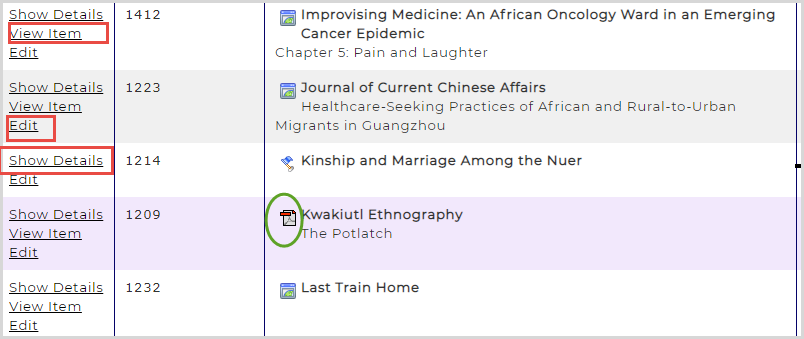
\includegraphics[width=\textwidth, height=6.5cm]{viewitem}
    \caption{Get More Info About Items}
    \label{fig:viewitem}
\end{figure}

\section{Use Tags to Organize}
\label{sec:tags}
Instructors and students can add tags to items on the \ares web interface so they can categorize them for easy viewing and organizing. There are two kinds of tags:
\subsection{Add Tags to A Single Item}
\begin{description}
    \item[Instructor Tags] These tags are visible to all instructors, proxies, and students in a course.
    \item[Personal Tags] They are for personal use and are not visible to anyone else.
\end{description}
To add tags:
\begin{enumerate}
    \item On the \ares web interface, open a \textbf{Course Details} page.
    \item Click \uline{Show Details} on a reserve Item you want to add a tag to.
    \item The \textbf{Reserve Item Details} page will open. It contains fields for entering Instructor and Personal Tags.
    \item Enter any desired Instructor or Personal Tags. \emph{The words and phrases used as \textbf{Tags need to be separated by a comma}}.
    \item Click \aresbut{ModifyTags} to save the list of tags.
    \item Click \uline{Back to [Course Name]} to go back to \textbf{Course Details} page.
\end{enumerate}

\vspace*{4ex}
\begin{figure}[h]
    \centering
    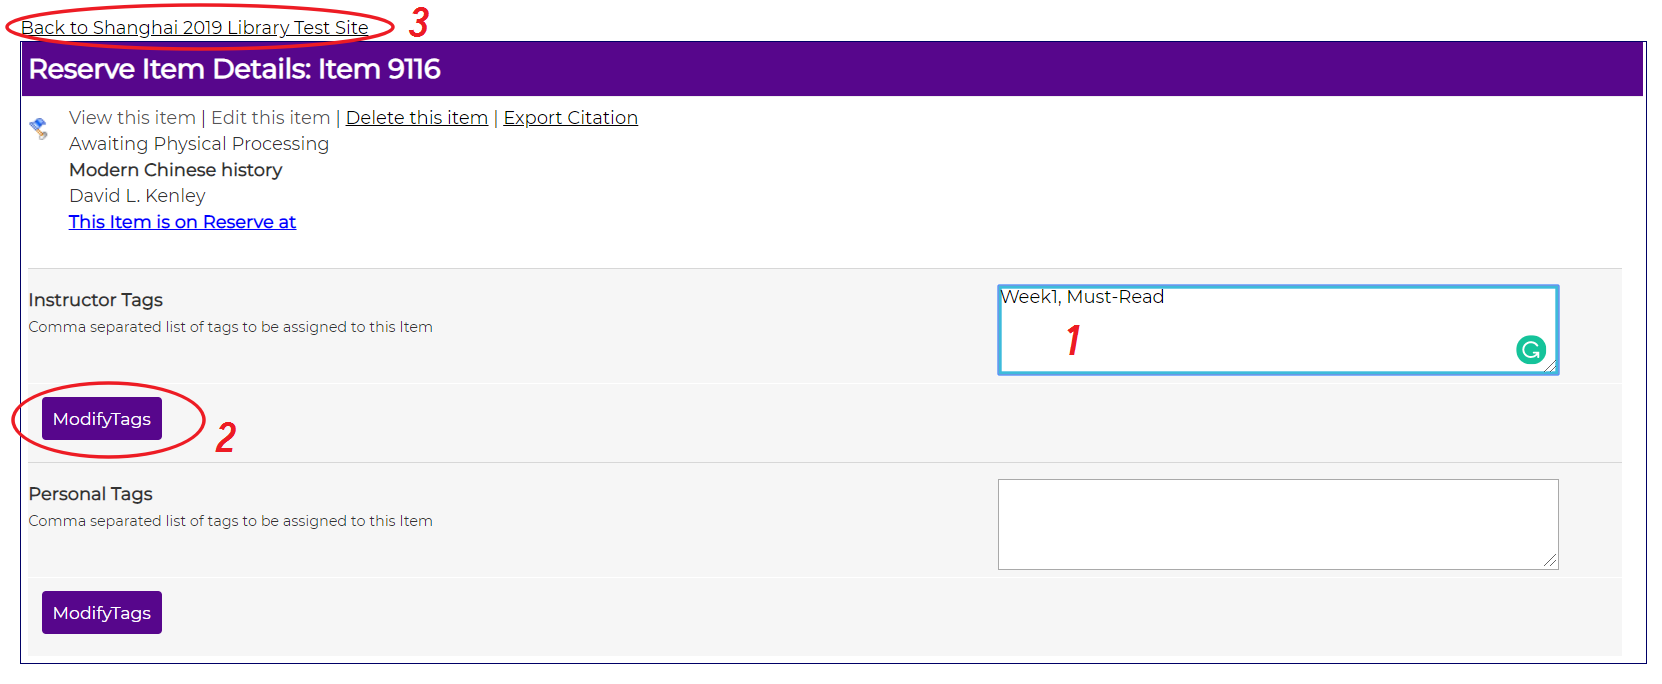
\includegraphics[width=\textwidth, height=7cm]{tag}
    \caption{Modify Tags}
    \label{fig:tag}
\end{figure}
\vspace*{2ex}

\subsection{Add Tags to A Group of Items}
Sometimes instructors need to group materials by, for example, subject or simply chronologically (e.g.\ Week1, Week2, ... etc.\ ). In \ares this need can be addressed by  \aresbut{Enable Batch Tag Editing}. Click on this button and add tags by following the steps shown in the pic below:
% \tcbdocmarginnote{\href{https://youtu.be/wUEl8KrMz14}{video tutorial}}
\vspace*{4ex}
\begin{figure}[h]
    \centering
    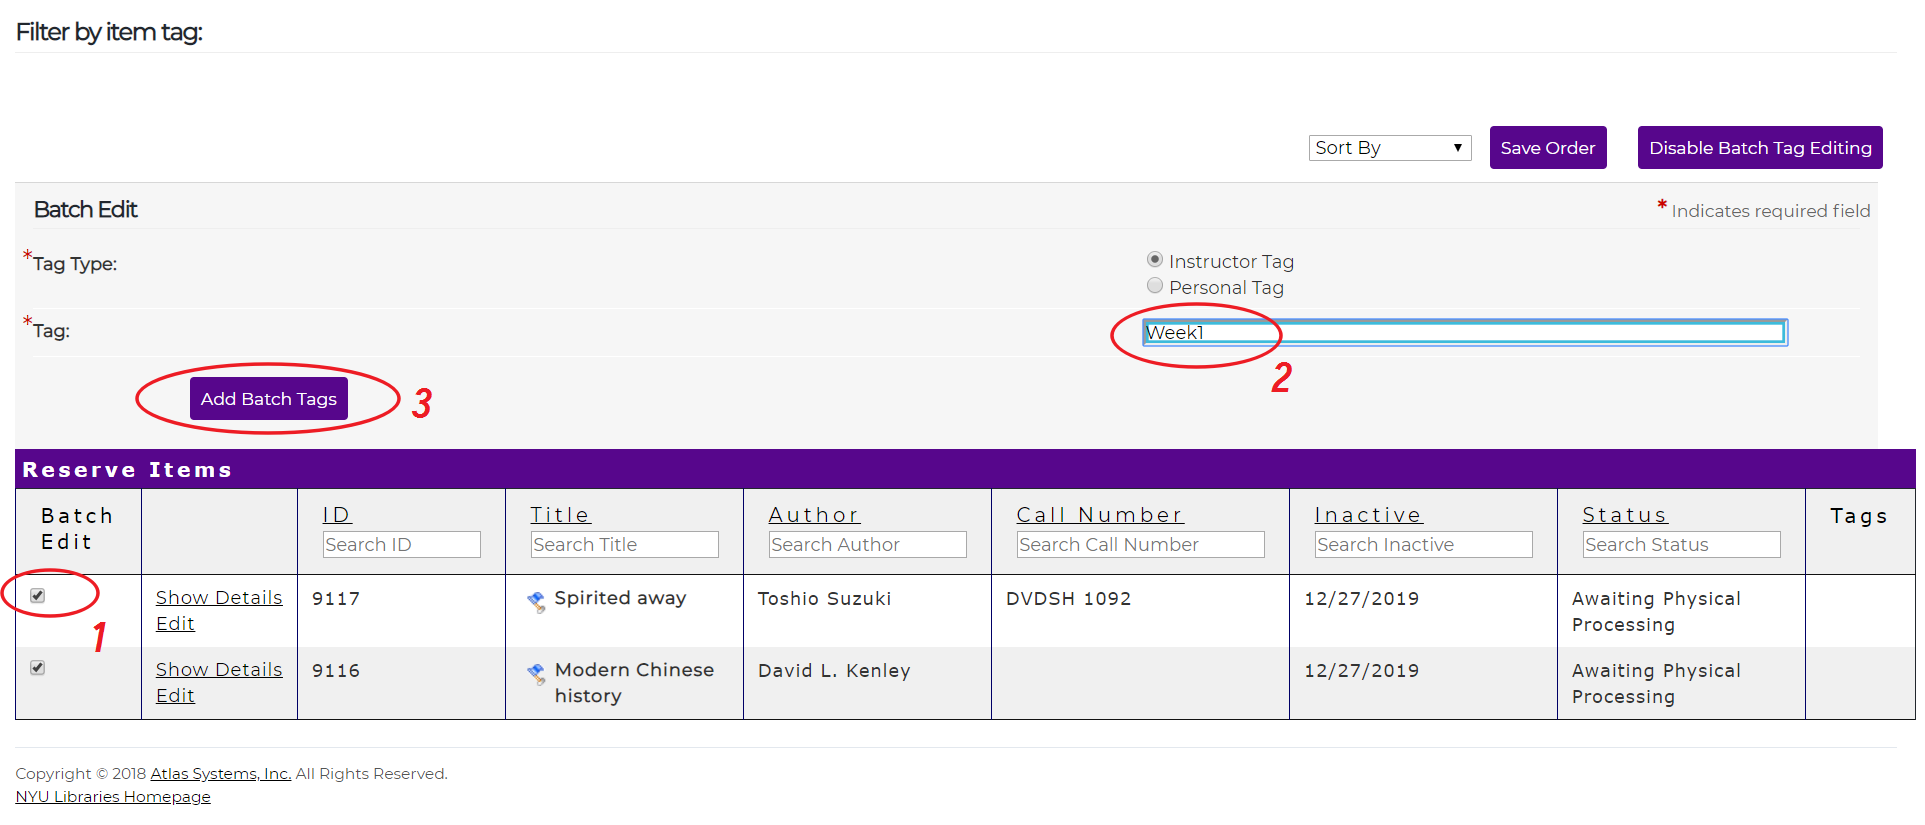
\includegraphics[width=\textwidth, height=6.5cm]{batchtag}
    \caption{Add Batch Tags}
    \label{fig:batchtag}
\end{figure}
\vspace*{2ex}

\section{Filter Items with Tags}
Once the tags have been added, instructors and students can filter their list of reserve Items by tag on a \textbf{Course Details} page:
\begin{itemize}
    \item Click on a tag from the list above the \textbf{Reserve Items} grid \textbf{or}
    \item Click on a tag link in the Tags column in the grid
\end{itemize}

Clicking on a tag will filter the view for that tag and show only Reserve Items containing that tag. The bracketed number following the tags show is the number of items labelled with that tag. To close a tag filter, click \uline{View all items for [Course Name]}.
\vspace*{4ex}
\begin{figure}[h]
    \centering
    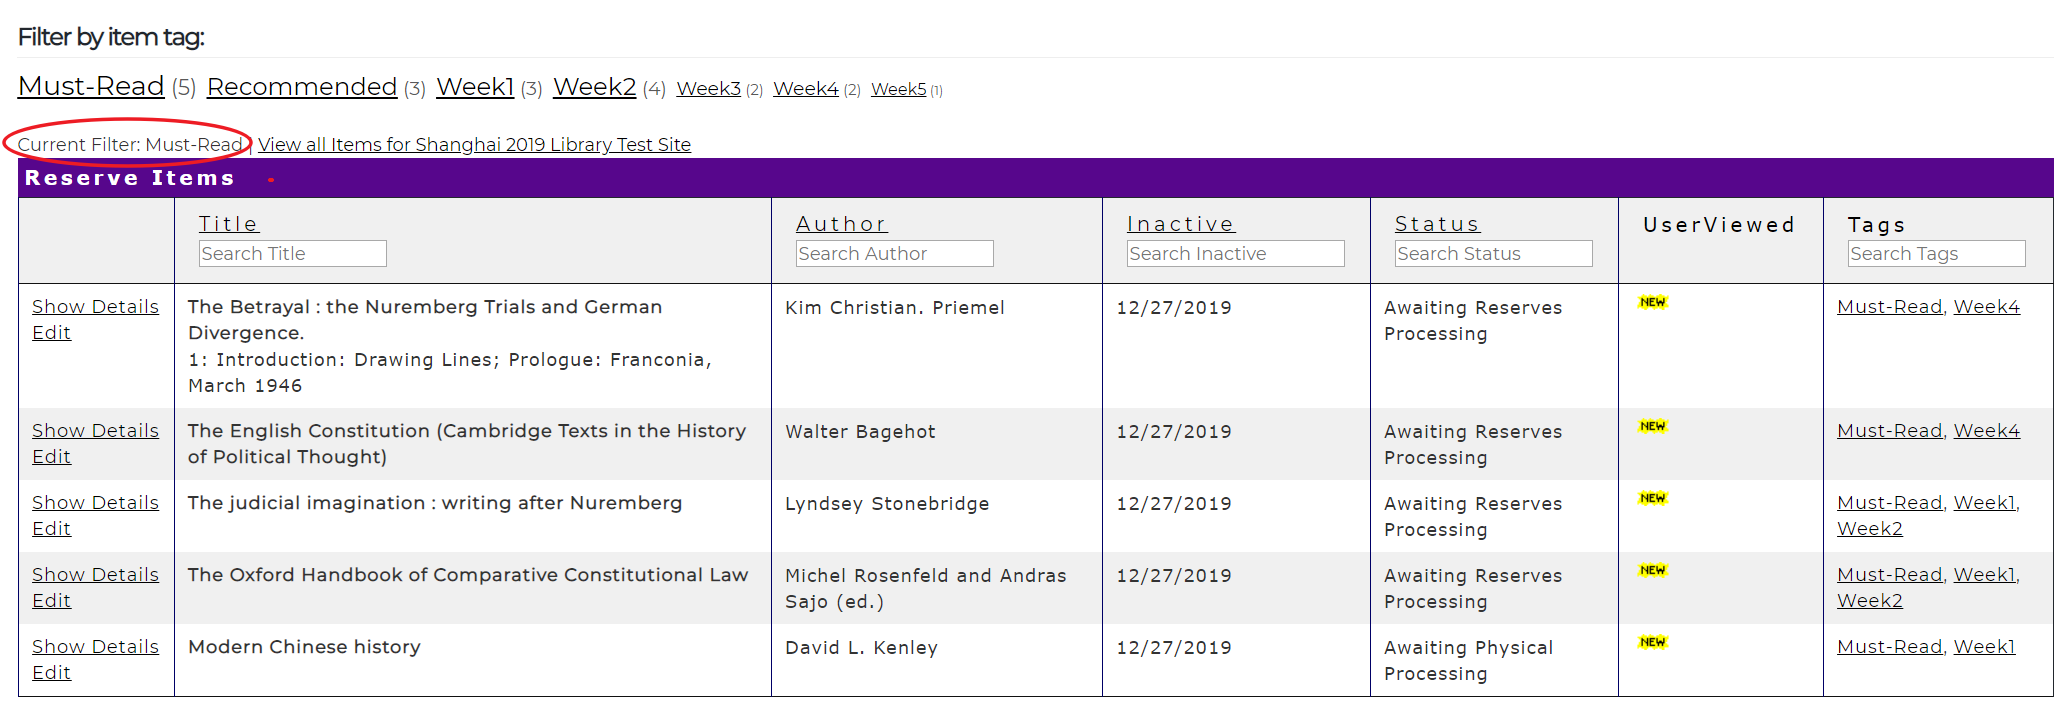
\includegraphics[width=\textwidth, height=5.5cm]{batchtag1}
    \caption{Filter Items Using Tags}
    \label{fig:filter}
\end{figure}







